
%%%%%%%%%%%%%%%%%% 插图环境 %%%%%%%%%%%%%%%%%%

\chapter{数值模拟}

接下来, 我们将通过Matlab数值模拟来验证所提数值方法的强收敛主要结论. 在本章中, 将呈现一维和二维的两个数值算例.
\begin{example}\label{ex}
    考虑一个一维时间变换随机微分方程
    \begin{align}\label{ex1}
        \left\{
        \begin{array}{lr}
            dY(t)=\left([t(1-t)]^{\frac{1}{4}}Y(t)-Y^5(t)\right)dE(t)+\left([t(1-t)]Y^2(t)\right)dW(E(t)),&\\
            Y(0)=1,&
        \end{array}
        \right.
    \end{align}
\end{example}
令$T=1$, 该方程中漂移项和扩散项系数分别为$f(y)=[t(1-t)]^{\frac{1}{4}}y-y^5$ 和 $g(y)=[t(1-t)]y^2$. 显然, 它们都具有连续的二阶导数, 并且不难验证当$\alpha =4$时,
假设\ref{ass1}和假设\ref{ass5}成立.
\par
对任意$p>2$有
\begin{align*}
    &(x-y)^{\mathrm{T}}(f(t,x)-f(t,y))+(5p-1)|g(t,x)-g(t,y)|^2\\
   =&(x-y)^T\bigg([t(1-t)]^{\frac{1}{4}}(x-y)-(x^5-y^5)\bigg)+(5p-1)\big|[t(1-t)](x^2-y^2)\big|^{2}\\
    \leq&
    (x-y)^2\bigg([t(1-t)]^{\frac{1}{4}}-(x^4+x^{3}y+x^{2}y^{2}+xy^{3}+y^4)+(5p-1)[t(1-t)]^{2}(x+y)^{2}\bigg).
\end{align*}
由于
\begin{align*}
    -(x^{3}y+xy^{3})=-xy(x^{2}+y^{2})\leq 0.5(x^{2}+y^{2})^{2}=0.5(x^{4}+y^{4})+x^{2}y^{2}.
\end{align*}
因此
\begin{align*}
    &(x-y)^{\mathrm{T}}(f(t,x)-f(t,y))+(5p-1)|g(t,x)-g(t,y)|^2\\
    \leq&(x-y)^2\bigg([t(1-t)]^{\frac{1}{4}}-0.5(x^4+y^4)+2(5p-1)[t(1-t)]^{2}(x^{2}+y^{2})\bigg)\\
    \leq& K(x-y)^{2}.
\end{align*}
这里使用了Young不等式. 最后一个不等式根据多项式的最高阶项系数为负系数时始终有界的性质得到, 因此假设$\ref{ass2}$成立.
\par
类似地, 对任意$q>2$和任意$t\in [0,1]$有
\begin{align*}
    & x^{\mathrm{T}}f(t,x)+(5q-1)|g(t,x)|^2\\
    =& [t(1-t)]^{\frac{1}{4}}x-x^5+(5q-1)[t(1-t)]^{2}x^4\\
    \leq & K_{1}(1+|x|^2).
\end{align*}
故假设\ref{ass3}成立.
\par
然后对方程中的时间变量使用均值定理, 假设\ref{ass4}在$\gamma_f=\frac{1}{4}$, $\gamma_g=1$时成立. 所以由定理\ref{theorem3-2}可得
\begin{align*}
    \EE \left( \sup_{0\leq t\leq T}|Y(t)-X(t)|^{\bar{p}} \right) \leq C\bigg(h^{\frac{\bar{p}}{4}}+h^{\bar{p}}+h^{\bar{p}}(\k(h))^{2\bar{p}}+\big(\mu^{-1}(\k(h))\big)^{5\bar{p}-q}\bigg)
\end{align*}
和
\begin{align*}
    \EE \left( \sup_{0\leq t\leq T}|Y(t)-\bar{X}(t)|^{\bar{p}} \right) \leq C\bigg(h^{\frac{\bar{p}}{4}}+h^{\bar{p}}+h^{\bar{p}}(\k(h))^{2\bar{p}}+\big(\mu^{-1}(\k(h))\big)^{5\bar{p}-q}\bigg).
\end{align*}
根据方程\ref{ex1}的漂移项和扩散项的系数, 易得到
\begin{align*}
    \sup_{0\leq t\leq 1}\sup_{|x|\leq u}(|f(t,x)|\vee |g(t,x)|\vee |Lg(t,x)|)\leq 2u^5,\quad  \forall u\geq 1.
\end{align*}
所以对任意$\varepsilon \in (0,1/4]$, 我们令$\m (u)=2u^5$ 和 $\k(h)=h^{-\varepsilon}$, 则有$\m^{-1}(u)=\left(u/2\right)^{1/5}$和 $\m^{-1}(\k(h))=\left(h^{-\varepsilon}/2\right)^{1/5}$. 当选择足够小的$\varepsilon$和足够大的$p$, 根据定理\ref{theorem3-1},可推导出
\begin{align*}
    \EE \left( \sup_{0\leq t\leq 1}|Y(t)-X(t)|^{\bar{p}} \right) \leq Ch^{\bar{p}/4}
\end{align*}
和
\begin{align*}
    \EE \left( \sup_{0\leq t\leq 1}|Y(t)-\bar{X}(t)|^{\bar{p}} \right) \leq Ch^{\bar{p}/4}.
\end{align*}
结论表明时间变换随机微分方程\eqref{ex1}的截断Milstein方法的收敛阶为$0.25$.
\par
接下来, 我们通过Matlab计算均方误差的近似值. 通过选择不同的步长$10^{-1}$、$10^{-2}$、 $10^{-3}$、 $10^{-4}$、 $10^{-5}$, 并对每个步长都模拟\eqref{findXn}的M=100条独立的轨迹. 我们选择 $\varepsilon=0.02$, 由于时间变换随机微分方程的真实解很难被显式表达, 故本文将步长为$10^{-5}$的数值解视为精确解, 画出其收敛图如下:
\begin{figure}[H]
    \centering
    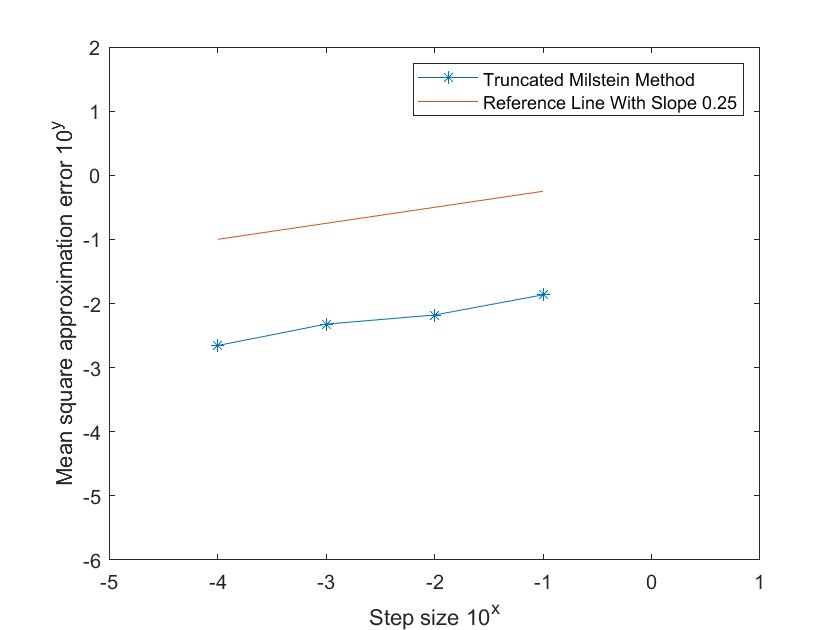
\includegraphics[width=0.70\textwidth]{11.jpg}
    \caption{例\ref{ex}的收敛率}
\end{figure}
从图4.1中不难看出, 截断Milstein的强收敛阶约为0.25. 我们通过Matlab数值模拟得出误差对步长的斜率为0.2517, 故验证了理论结果.

\begin{example}\label{exp}
   考虑一个二维时间变换随机微分方程
    \begin{align}
        \label{ex2}
        \left\{
        \begin{array}{lr}
            dx_1(t)=\left([t(1-t)]^{\frac{1}{5}}x_1(t)-x_2^5(t)\right)dE(t)+\left([t(1-t)]^{\frac{1}{2}}x_2^2(t)\right)dW(E(t)),&\\
            dx_2(t)=\left([t(1-t)]^{\frac{1}{5}}x_2(t)-x_1^5(t)\right)dE(t)+\left([t(1-t)]^{\frac{1}{1}}x_1^2(t)\right)dW(E(t)).&
        \end{array}
        \right.
    \end{align}
\end{example}
其中
\begin{align*}
    f(t,x)=
    \begin{pmatrix}
        [t(1-t)]^{\frac{1}{5}}x_1-x_2^5\\
        [t(1-t)]^{\frac{1}{5}}x_2-x_1^5
    \end{pmatrix}
    ~~~~~\text{和}~~~~~
    g(t,x)=
    \begin{pmatrix}
        [t(1-t)]^{\frac{1}{2}}x_2^2\\
        [t(1-t)]^{\frac{1}{2}}x_1^2
    \end{pmatrix}.
\end{align*}
类似例4.1, 不难验证系数$f(t,x)$ 和 $g(t,x)$满足假设\ref{ass1}和\ref{ass5}, 其中$\a=4$. 对任意$x,y\in\RR$, 容易得到
\begin{align*}
    &(x-y)^{\mathrm{T}}(f(t,x)-f(t,y))+(5p-1)|g(t,x)-g(t,y)|^2\\
    = & (x_1-y_1)\bigg([t(1-t)]^{\frac{1}{5}}(x_1-y_1)-(x_2^5-y_2^{5})\bigg)+(x_2-y_2)\bigg([t(1-t)]^{\frac{1}{5}}(x_2-y_2)\\
    \quad &-(x_1^5-y_1^{5})\bigg)+(5p-1)\bigg([t(1-t)]^{\frac{1}{2}}(x_2^2-y_2^2)^2
    +[t(1-t)]^{\frac{1}{2}}(x_1^2-y_1^2)\bigg)^2\\
    \leq & (x_1-y_1)^2\left([t(1-t)]^{\frac{1}{5}}-(x_2^4+x_2^3y_2+x_2^2y_2^2+x_2y_2^3+y_2^4)\right)\\
    \quad &+(x_2-y_2)^2\left([t(1-t)]^{\frac{1}{5}}-(x_1^4+x_1^3y_1+x_1^2y_1^2+x_1y_1^3+y_1^4)\right)\\
    \quad &+2(5p-1)\bigg([t(1-t)](x_2^2-y_2^2)^2+[t(1-t)](x_1^2-y_1^2)^2\bigg)\\
    \leq & (x_1-y_1)^2\left([t(1-t)]^{\frac{1}{5}}-(x_2^4+x_2^3y_2+x_2^2y_2^2+x_2y_2^3+y_2^4)\right)\\
    \quad &+(x_2-y_2)^2\bigg([t(1-t)]^{\frac{1}{5}}-(x_1^4+x_1^3y_1+x_1^2y_1^2+x_1y_1^3+y_1^4)\bigg)\\
    \quad &+2(x_2-y_2)^{2}(5p-1)\bigg([t(1-t)](x_2+y_2)^2\bigg)+2(x_1-y_1)^{2}(5p-1)\\
    & \times\bigg([t(1-t)](x_1+y_1)^2\bigg).
\end{align*}
由于
\begin{align*}
    -(x^3y+xy^3)=-xy(x^2+y^2)\leq 0.5(x^2+y^2)^2=0.5(x^4+y^4)+x^2y^2.
\end{align*}
故对任意$t\in[0,1]$有
\begin{align*}
    &(x-y)^{\mathrm{T}}(f(t,x)-f(t,y))+(5p-1)|g(t,x)-g(t,y)|^2\\
    \leq &(x_1-y_1)^2\bigg([t(1-t)]^{\frac{1}{5}}-0.5(x_2^4+y_2^4)+2(5p-1)[t(1-t)](x_1+y_1)^{2}\bigg)\\
    &+(x_2-y_2)^2\bigg([t(1-t)]^{\frac{1}{5}}-0.5(x_1^4+y_1^4)+2(5p-1)[t(1-t)](x_2+y_2)^{2}\bigg)\\
    \leq &C(x-y)^2,
\end{align*}
这里使用了基本不等式$(a+b)^{2}\leq 2(a^{2}+b^{2})$以及多项式的最高阶项系数为负系数时始终有界的性质, 故假设$\ref{ass2}$成立.
\par
对任意$q>2$和$t\in[0,1]$, 下面推导假设\ref{ass3}是成立的.
\begin{align*}
    & x^{\mathrm{T}}f(t,x)+(5q-1)|g(t,x)|^2\\
    =& ([t(1-t)]^{\frac{1}{5}}x_1^2-x_1x_2^5)+([t(1-t)]^{\frac{1}{5}}x_2^2-2x_1^5x_2)+2(5q-1)|[t(1-t)](x_1^{2}+x_2^{2})|^2\\
    \leq & [t(1-t)]^{\frac{1}{5}}(x_1^2+x_2^2)-x_1x_2(x_1^4+x_2^4)+2(5q-1)[t(1-t)](x_1^2+x_2^2)\\
    \leq & C(1+|x|^2).
\end{align*}
由于$\gamma_f\in (0,1]$ 和$\gamma_g\in (0,1]$, 对任意$s,t\in[0,T]$, 我们通过对时间变量使用均值定理, 即
\begin{align*}
    &|f(s,x)-f(t,x)|\\
    \leq& \big|([(s(1-s)]^{\frac{1}{5}}-[t(1-t)]^{\frac{1}{5}})x_1+([s(1-s)]^{\frac{1}{5}}-[t(1-t)]^{\frac{1}{5}})x_2\big|\\
    \leq& C_1|s-t|^{\frac{1}{5}}x_1+C_2|s-t|^{\frac{1}{5}}x_2
\end{align*}
和
\begin{align*}
    &|g(s,x)-g(t,x)|\\
    \leq& \big|([s(1-s)]^{\frac{1}{2}}-[t(1-t)]^{\frac{1}{2}})x_2^2+([s(1-s)]^{\frac{1}{2}}-[t(1-t)]^{\frac{1}{2}})x_1^2\big|\\
    \leq& C_1|s-t|^{\frac{1}{2}}x_2^2+C_2|s-t|^{\frac{1}{2}}x_1^2.
\end{align*}
可得假设\ref{ass4}在$\gamma_f=1/5$ 和 $\gamma_g=1/2$时成立. 再根据定理\ref{theorem3-2}和例\ref{ex}, 对任意$\varepsilon \in (0,1/4]$, 我们令$\m (u)=2u^5$ 和 $\k(h)=h^{-\varepsilon}$, 当选择足够小$\varepsilon$和足够大的$p$时, 根据定理\ref{theorem3-1}可得

\begin{align*}
    \EE \left( \sup_{0\leq t\leq 1}|Y(t)-X(t)|^{\bar{p}} \right) \leq Ch^{\bar{p}/5}
\end{align*}
和
\begin{align*}
    \EE \left( \sup_{0\leq t\leq 1}|Y(t)-\bar{X}(t)|^{\bar{p}} \right) \leq Ch^{\bar{p}/5}.
\end{align*}
\par
上面结论表明了时间变换随机微分方程\eqref{ex2}截断Milstein方法的收敛阶为$1/5$.同样地, 接下来我们将通过计算机模拟进行验证.
\par 
同例\ref{ex}, 我们对\eqref{findXn}选取不同步长 $10^{-1}$、$10^{-2}$、$10^{-3}$、$10^{-4}$、$10^{-5}$ ,然后对每个步长都模拟M=100条独立轨迹, 将步长为$10^{-5}$的数值解视为精确解, 画出其收敛图如下:
\begin{figure}[H]
    \centering
    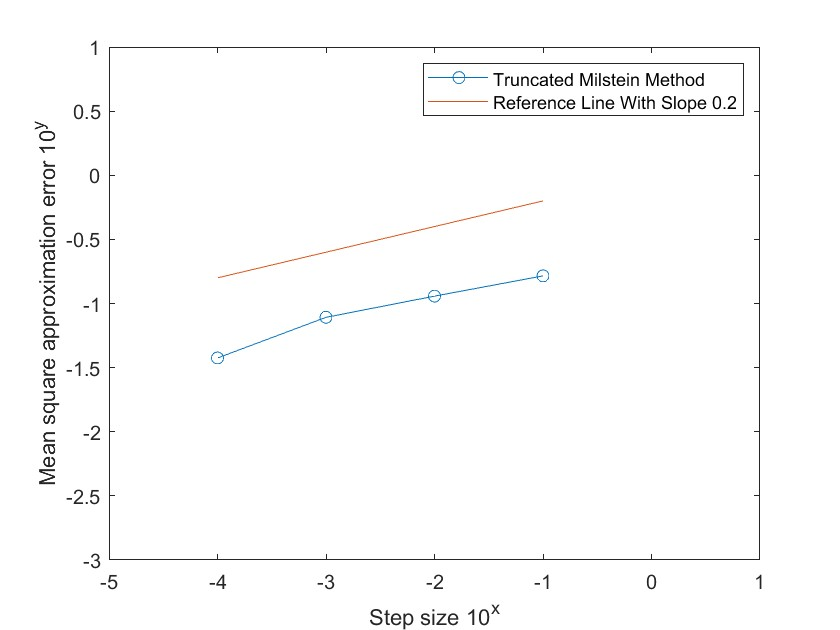
\includegraphics[width=0.70\textwidth]{22.jpg}
    \caption{例子\ref{exp}的收敛率}
\end{figure}
从图4.2不难看出收敛阶约为0.2. 我们通过应用线性回归得出误差线的斜率约为0.2086, 其与理论结果非常接近, 同样验证了本文的重要结论.

